\otazka{4. Sítě a síťové aplikace}{Modely vrstev počítačových sítí (ISO/OSI, TCP/IP), funkcionalita a součinnost vrstev, adresace. Fyzická vrstva, signály a jejich kódování, řízení přístupu k médiu. Propojování počítačových sítí. Síťové protokoly, přepínání a směrování, multicast. Zajištěný přenos dat, sestavení a ukončení spojení. Transportní protokoly. Základní aplikační protokoly: doručování pošty, přenos souborů, web, jmenná služba. Principy popisu a zajištění kvality služby, použití pro multimédia. Zabezpečení síťové komunikace, autentizace a šifrování, zabezpečení na jednotlivých protokolových vrstvách.}{PB156, PB156cv}

\subsection*{4. Sítě -- stručněji}
Síť je systém, ve kterém zařízení komunikují pomocí vrstev, adres a protokolů. Dobrá odpověď má ukázat cestu dat: aplikace vytvoří zprávu, transport ji doručuje procesu, IP síť ji směruje mezi sítěmi, linková vrstva ji předá dalšímu hopu a fyzická vrstva ji pošle jako signál.

\textbf{1. Vrstvy a jejich smysl}
\begin{itemize}
  \item ISO/OSI je sedmivrstvý referenční model, TCP/IP je praktičtější internetový model. Smysl vrstev je oddělit odpovědnosti a skrýt detaily nižších vrstev.
  \item Zkoušková věta: L7 řeší význam zprávy, L4 porty a procesy, L3 IP adresy a směrování, L2 rámce a sousední uzel, L1 fyzický signál.
\end{itemize}

\textbf{2. Adresace}
\begin{itemize}
  \item MAC adresa je linková a platí v lokální síti. IP adresa je síťová a slouží k doručení přes více sítí. Port určuje aplikaci nebo proces na koncovém zařízení.
  \item Privátní IPv4 rozsahy jsou 10.0.0.0/8, 172.16.0.0/12 a 192.168.0.0/16. Do Internetu se přímo nesměrují a typicky se používají za NATem.
\end{itemize}

\textbf{3. Fyzická a linková vrstva}
\begin{itemize}
  \item Fyzická vrstva řeší médium, signál, kódování a přenos bitů. Linková vrstva řeší rámce, MAC adresy, detekci chyb a přístup k médiu.
  \item Ethernet dnes typicky používá switche a full-duplex, takže staré kolize přes huby už nejsou běžný model moderní LAN.
\end{itemize}

\textbf{4. Přepínání a směrování}
\begin{itemize}
  \item Switch přepíná rámce podle MAC adres v jedné síti. Router směruje pakety podle IP adres mezi sítěmi.
  \item ARP mapuje IPv4 adresu na MAC adresu v lokální síti. DNS naopak mapuje jména na IP adresy a patří aplikačně výš.
\end{itemize}

\textbf{5. Transport}
\begin{itemize}
  \item TCP poskytuje spojovaný, spolehlivý a seřazený přenos s potvrzováním, řízením toku a zahlcení. Spojení se sestavuje třícestným handshake.
  \item UDP je jednodušší a bez záruk doručení. Hodí se tam, kde aplikace chce nižší režii nebo si spolehlivost řeší sama, například DNS, VoIP nebo hry.
  \item Multicast je doručení skupině příjemců, ne všem jako broadcast a ne jednomu jako unicast.
\end{itemize}

Modely vrstev počítačových sítí (\textbf{ISO/OSI}, \textbf{TCP/IP}), funkcionalita a součinnost vrstev, adresace, fyzická a linková vrstva, propojování sítí, síťové protokoly, přepínání, \textbf{směrování}, \textbf{multicast}, zajištěný přenos a transportní protokoly.

\subsection*{Tento text je psaný jako souvislé opakování ke státnicím: cílem není jen vyjmenovat pojmy, ale umět mluvit o tom, co se s daty reálně děje při průchodu sítí. Zkouškově nejdůležitější osa je: L7 význam zprávy, L4 porty/procesy, L3 IP a směrování, L2 rámec a další hop, L1 signál.}

\subsection*{1. Základní představa: co je síť a proč jsou vrstvy}

Počítačová síť je skupina zařízení propojených komunikačními kanály, která umožňuje přenos dat a sdílení zdrojů. U přenosu sledujeme hlavně doručení, správnost a včasnost doručení. Kvalitu toku popisuje propustnost, ztrátovost paketů, \textbf{latence} a \textbf{jitter}. Propustnost říká, kolik dat se reálně přenese za sekundu; latence je zpoždění; jitter je kolísání zpoždění; ztrátovost říká, jaká část paketů nedorazí.

Protokol určuje syntaxi, sémantiku a časování komunikace: tedy jak zprávy vypadají, co znamenají a kdy se posílají.

Vrstvení existuje proto, aby se složitý problém rozdělil na menší části. Každá vrstva poskytuje službu vrstvě nad sebou, používá službu vrstvy pod sebou a při odesílání přidává vlastní řídicí informace. Při příjmu se postupuje opačně. Logicky spolu komunikují stejné vrstvy na obou koncích, ale fyzicky data vždy projdou přes nižší vrstvy.

Příjem: L1 signál -> L2 \textbf{rámec} -> L3 \textbf{paket} -> L4 \textbf{segment} -> L7 data

\subsection*{2. ISO/OSI a TCP/IP}

ISO/OSI je sedmivrstvý referenční model. Je užitečný hlavně pro vysvětlení funkcí vrstev a pro slovník typu L1, L2, L3. \textbf{TCP}/IP je praktický model Internetu. V TCP/IP se L5 až L7 typicky sloučí do aplikační vrstvy, L4 odpovídá transportní vrstvě, L3 internetové vrstvě a L1-L2 vrstvě síťového rozhraní.

Důvod je praktický: různé aplikace potřebují různé formáty, šifrování, relace a aplikační pravidla, takže si tyto funkce v TCP/IP často řeší aplikace, knihovny a aplikační protokoly.

\begin{longtable}{p{0.237\linewidth}p{0.237\linewidth}p{0.237\linewidth}p{0.237\linewidth}}
\toprule
\textbf{OSI} & \textbf{Funkce} & \textbf{TCP/IP pohled} & \textbf{Příklady} \\
\midrule\endhead
L7 aplikační & Význam aplikační komunikace: co si aplikace říkají. & Aplikační & HTTP, DNS, SMTP, IMAP, FTP, SSH \\
\addlinespace
L6 prezentační & Reprezentace dat: kódování, serializace, komprese, šifrování. & Aplikační & UTF-8, JSON/XML, gzip, TLS funkce \\
\addlinespace
L5 relační & Relace/dialog: stav komunikace, session, checkpointy. & Aplikační & TLS session, webová session, SSH session \\
\addlinespace
L4 transportní & Komunikace mezi procesy, porty, TCP/UDP, spolehlivost. & Transportní & TCP segment, UDP datagram \\
\addlinespace
L3 síťová & Doručení mezi sítěmi, IP adresy, směrování. & Internetová & IPv4/IPv6, ICMP, IGMP, ARP jako podpůrný mechanismus \\
\addlinespace
L2 linková & Doručení na jednom úseku, rámce, MAC, přístup k médiu. & Síťové rozhraní & Ethernet, Wi-Fi, switch \\
\addlinespace
L1 fyzická & Bity jako signál v médiu. & Síťové rozhraní & Kabel, optika, rádio, kódování signálu \\
\addlinespace
\bottomrule
\end{longtable}

\itzk{\textbf{Poznámka ke zkoušce:} když se řekne L1/L2/L3, jde obvykle o OSI číslování. V praxi se ale tato označení běžně používají i při popisu TCP/IP sítí.}

\subsection*{3. Co dělají vrstvy při reálném odeslání dat}

Při otevření webu aplikace nejprve vytvoří aplikační zprávu, například \textbf{HTTP} požadavek. Prezentační funkce ji převedou do společné podoby: text do \textbf{UTF-8}, objekt na JSON/XML, případně komprese nebo šifrování. Relační funkce drží kontext komunikace, například \textbf{TLS} session nebo webovou session. Transportní vrstva přidá porty a u TCP zajišťuje spolehlivý proud bajtů.

Síťová vrstva přidá IP adresy a řeší, kam má paket dojít celkově. Linková vrstva zabalí IP paket do rámce pro jeden konkrétní úsek cesty. Fyzická vrstva rámec převede na bity/signál.

HTTP request -> TCP segment: zdrojový port 51544, cílový port 443 -> IP paket: zdrojová IP, cílová IP serveru -> \textbf{Ethernet}/Wi-Fi rámec: zdrojová \textbf{MAC}, cílová MAC dalšího hopu -> elektrický/optický/rádiový signál

Zásadní rozdíl: IP adresa označuje konečný stroj nebo rozhraní v síťové vrstvě, zatímco MAC adresa u Ethernetu/Wi-Fi řeší jen aktuální linkový úsek. Když je server mimo lokální síť, počítač nevkládá do rámce MAC adresu serveru, ale MAC adresu default gateway. Router rámec přijme, odstraní L2 obal, podívá se na cílovou IP, zvolí další hop, vytvoří nový L2 rámec a pošle paket dál.

Proto je dobré být přesný: samotná IP komunikace je logicky mezi zdrojovým a cílovým uzlem (end-to-end), ale rozhodování o cestě probíhá hop-by-hop, tedy na každém routeru zvlášť. Na každém hopu navíc vzniká nový linkový rámec a MAC adresy v něm platí jen pro daný linkový úsek, ne pro celou cestu.

\subsection*{Zkoušková věta: L3 řekne, kam to má dojít celkově; L2 řekne, komu to předám právě teď; L1 řekne, jak to fyzicky pošlu.}

\subsection*{4. Adresace: MAC, IP, port}

Na L2 se u Ethernetu a Wi-Fi používá MAC adresa, typicky zapisovaná jako šest bajtů v hexadecimálním tvaru. Patří síťovému rozhraní a slouží pro lokální doručení rámce. Na L3 se používá IP adresa. IPv4 má 32 bitů, IPv6 má 128 bitů. IP adresa se používá pro doručení mezi sítěmi a pro směrování. Na L4 jsou porty, 16bitová čísla, která identifikují aplikaci nebo službu na konkrétním uzlu.

Aplikace v komunikaci se prakticky identifikuje dvojicí IP adresa:port.

\begin{longtable}{p{0.237\linewidth}p{0.237\linewidth}p{0.237\linewidth}p{0.237\linewidth}}
\toprule
\textbf{Vrstva} & \textbf{Adresace} & \textbf{Datová jednotka} & \textbf{Co znamená} \\
\midrule\endhead
L2 & MAC / linková adresa & rámec & Komu to předám na tomto úseku, např. počítač -> router. \\
\addlinespace
L3 & IP adresa & paket/datagram & Kam to má dojít přes sítě, např. na cílový server. \\
\addlinespace
L4 & port & segment/datagram & Kterému procesu/službě na stroji to patří. \\
\addlinespace
\bottomrule
\end{longtable}

IPv4 adresace se historicky dělila do tříd, ale dnes je důležitější classless adresování, masky a \textbf{CIDR}. Maska říká, která část adresy je síťová a která hostitelská; adresa sítě vzniká jako IP AND maska.

Subnetting dělí síť na podsítě, \textbf{supernetting}/agregace spojuje sousední bloky kvůli menším směrovacím tabulkám. \textbf{NAT} překládá privátní adresy a porty na veřejnou adresu, takže více zařízení v domácí síti může sdílet jednu veřejnou IPv4 adresu.

\itbox{\textbf{Privátní IPv4 rozsahy podle RFC 1918:} do Internetu se přímo nesměrují a typicky se používají za NATem. Rychlá pomůcka je pamatovat si tři starty: \textbf{10, 172, 192}.}

\begin{longtable}{p{0.22\linewidth}p{0.25\linewidth}p{0.46\linewidth}}
\toprule
\textbf{Pomůcka} & \textbf{CIDR rozsah} & \textbf{Jak si to zapamatovat} \\
\midrule\endhead
\textbf{Obří krabice} & \texttt{10.0.0.0/8} & Jakmile IPv4 adresa začíná na \textbf{10.}, je privátní. Hodí se pro velké organizace, laboratoře nebo rozsáhlé interní sítě. \\
\addlinespace
\textbf{Střední firemní krabice} & \texttt{172.16.0.0/12} & Začíná na \textbf{172.16.} až \textbf{172.31.}. Nestačí vidět číslo 172 někde v adrese; rozhoduje začátek a rozsah druhého oktetu 16--31. \\
\addlinespace
\textbf{Domácí krabice} & \texttt{192.168.0.0/16} & Klasické domácí routery: například \texttt{192.168.0.1} nebo \texttt{192.168.1.1}. Privátní je ale právě \textbf{192.168.*.*}, ne libovolná adresa začínající 192. \\
\bottomrule
\end{longtable}

\itpr{\textbf{Rychlý test:} \texttt{8.8.8.8} nezačíná na 10, 172.16--31 ani 192.168, takže je veřejná. \texttt{77.75.75.172} má sice na konci 172, ale nezačíná privátním rozsahem, takže je veřejná. \texttt{10.150.12.3} začíná na 10, takže je privátní.}

IPv6 rozšiřuje adresní prostor, nemá \textbf{broadcast} a místo něj používá multicastové skupiny; přidává také \textbf{anycast}, kde se data doručí nejbližšímu členovi skupiny.

\textbf{ARP} slouží u IPv4 ke zjištění MAC adresy pro známou IP adresu v lokální síti. Pokud chce host poslat paket na IP v jiné síti, nehledá MAC cílového serveru, ale MAC své default gateway. Pošle ARP request broadcastem: kdo má IP 192.168.1.1? Odpoví pouze zařízení s touto IP a pošle ARP reply se svou MAC adresou.

Aby host vůbec mohl komunikovat, potřebuje IP adresu a další parametry. Ty obvykle nezadává člověk ručně, ale přidělí je \textbf{DHCP} server. Průběh se shrnuje zkratkou \textbf{DORA}:
\begin{enumerate}
  \item \textbf{Discover} -- klient pošle broadcastem dotaz, kterým hledá DHCP server.
  \item \textbf{Offer} -- server nabídne adresu.
  \item \textbf{Request} -- klient o nabídnutou adresu požádá.
  \item \textbf{Acknowledge} -- server přidělení potvrdí.
\end{enumerate}

DHCP klientovi typicky předá IP adresu, masku sítě, výchozí bránu (gateway) a adresy \textbf{DNS} serverů. Adresa se přiděluje na omezenou dobu, takzvanou lease, kterou si klient před vypršením obnovuje.

Protože úvodní Discover je broadcast a ten se nešíří přes \textbf{router} do jiné podsítě, používá se v takovém případě DHCP relay: router nebo jiné zařízení DHCP požadavek zachytí a přepošle ho unicastem na centrální DHCP server v jiné síti.

\subsection*{5. Fyzická vrstva: signály, média a kódování}

Fyzická vrstva zajišťuje přenos jednotlivých bitů přes médium. Neřeší adresy ani význam dat. Řeší kódování bitů na signál, přenosovou rychlost, synchronizaci bitů, \textbf{multiplexing} a konkrétní fyzické médium. Média mohou být vedená, například kroucená dvojlinka, koaxiál nebo optické \textbf{vlákno}, nebo nevedená, například vzduch u rádiového přenosu. Signál je časová změna fyzikální veličiny.

Může slábnout, být zkreslený nebo rušený šumem. Digitální data se mohou přenášet digitálním signálem nebo modulací analogového nosného signálu.

Zásadní problém kódování je synchronizace vysílače a přijímače. Přijímač musí poznat, kde začínají a končí bity. Dlouhé posloupnosti stejných hodnot jsou problém, protože v signálu nemusí být dost změn pro synchronizaci hodin.

\begin{longtable}{p{0.237\linewidth}p{0.237\linewidth}p{0.237\linewidth}p{0.237\linewidth}}
\toprule
\textbf{Kódování} & \textbf{Princip} & \textbf{Výhoda} & \textbf{Nevýhoda} \\
\midrule\endhead
Přímé & Např. 1 je kladná amplituda, 0 nulová. & Jednoduché. & Není samosynchronizační. \\
\addlinespace
NRZ-L & Hodnota bitu je dána úrovní signálu. & Efektivní, jednoduché. & Dlouhé série stejných bitů kazí synchronizaci. \\
\addlinespace
NRZ-I & 1 znamená změnu polarity, 0 žádnou změnu. & Lepší práce se změnami. & Série nul bez změny je problém. \\
\addlinespace
\bottomrule
\end{longtable}

\begin{longtable}{p{0.237\linewidth}p{0.237\linewidth}p{0.237\linewidth}p{0.237\linewidth}}
\toprule
\textbf{Kódování} & \textbf{Princip} & \textbf{Výhoda} & \textbf{Nevýhoda} \\
\midrule\endhead
Manchester & Každý bit má přechod uprostřed bitového intervalu. & Plně samosynchronizační. & Na bit potřebuje dva signálové prvky, snižuje efektivní kapacitu. \\
\addlinespace
4B/5B & Čtyři bity se nahradí pětibitovým kódem s omezením dlouhých nul. & Lepší synchronizace, určitá detekce chyb. & Režie navíc; podobně fungují 8B/10B nebo 64B/66B. \\
\addlinespace
\bottomrule
\end{longtable}

\itbox{\textbf{Manchester pro 010:} vždy řekni konvenci. Pokud vezmu konvenci 0 = low-high a 1 = high-low, potom 010 = LH | HL | LH. U opačné konvence se výsledek převrátí.}

Multiplexing znamená sdílení kapacity média více komunikacemi. U analogových signálů jde například o \textbf{FDM}, kde má každý kanál jinou frekvenci, nebo \textbf{WDM} v optice, kde různé vlnové délky světla představují různé kanály. U digitálních signálů je typické \textbf{TDM}, kde se médium rozděluje v čase.

\subsection*{6. Linková vrstva a řízení přístupu k médiu}

Linková vrstva zajišťuje doručení rámce mezi sousedními uzly na jednom linkovém úseku. Vytváří rámce, používá linkové adresy, například MAC adresy u Ethernetu a Wi-Fi, může řešit detekci chyb, řízení toku a hlavně přístup ke sdílenému médiu. MAC v tomto kontextu znamená Medium Access Control: pravidla, která brání tomu, aby více stanic vysílalo do sdíleného média zároveň a rušilo se.

U Ethernetu má rámec pevnou strukturu, kterou je dobré umět vyjmenovat. Začíná preambulí a oddělovačem SFD (Start Frame Delimiter), tedy sledem bitů, který slouží k synchronizaci přijímače a označení začátku rámce. Následuje cílová MAC adresa a zdrojová MAC adresa, tedy komu rámec na tomto úseku patří a kdo ho poslal. Pole \textbf{EtherType} (případně délka) říká, jaký protokol je uvnitř, typicky IPv4, IPv6 nebo ARP.

Pak přichází payload, tedy přenášená data vyšší vrstvy, například IP paket. Rámec končí polem \textbf{FCS}, což je \textbf{CRC} kontrolní součet, kterým příjemce ověří, že se rámec cestou nepoškodil; pokud kontrola nesedí, rámec se zahodí.

\textbf{Aloha} dovolí stanici vysílat, kdykoliv má rámec, a při kolizi čeká náhodnou dobu a zkouší znovu. \textbf{CSMA/CD} je typické pro starší sdílený kabelový Ethernet s huby: stanice nejdřív poslouchá, zda je médium volné, při vysílání detekuje kolizi a pak zkusí po náhodné době znovu. Dnes u přepínaného full-duplex Ethernetu kolize prakticky neřešíme stejně jako dřív. \textbf{CSMA/CA} se používá u Wi-Fi: stanice se snaží kolizím předcházet, protože v rádiovém médiu nemůže spolehlivě současně vysílat a poslouchat.

\begin{longtable}{p{0.317\linewidth}p{0.317\linewidth}p{0.317\linewidth}}
\toprule
\textbf{Mechanismus} & \textbf{Kde/představa} & \textbf{Podstata} \\
\midrule\endhead
Aloha & Jednoduché sdílené médium & Vysílám kdykoliv, při kolizi opakuji. \\
\addlinespace
CSMA/CD & Starší kabelový Ethernet/huby & Poslouchám médium, vysílám při volnu, detekuji kolizi. \\
\addlinespace
CSMA/CA & Wi-Fi & Kolizím se snažím předcházet, typicky s čekáním/ACK. \\
\addlinespace
Polling/token/rezer vace & Řízený přístup & Vysílá ten, kdo dostane právo, token nebo časový interval. \\
\addlinespace
\bottomrule
\end{longtable}

Topologie sítě popisuje fyzické nebo logické uspořádání stanic: sběrnice, kruh a hvězda. U sběrnice a kruhu může výpadek média shodit velkou část sítě a \textbf{kolizní doména} je společná. Hvězda s centrálním prvkem je běžnější; u hubu jsou všechny stanice v jedné kolizní doméně, u switche se provoz odděluje podle portů.

\subsection*{7. Propojování sítí: hub, switch, bridge, router, gateway}

Síťová zařízení se často rozlišují podle vrstvy, na které primárně pracují. Opakovač a \textbf{hub} jsou L1 prvky: opakují signál a nerozumí rámcům. Bridge a \textbf{switch} jsou L2 prvky: pracují s MAC adresami a rámci. Switch je v podstatě víceportový \textbf{bridge}; učí se, na kterém portu je jaká MAC adresa, podle zdrojových adres přijatých rámců.

Router je L3 prvek: propojuje různé sítě a podle cílové IP adresy vybírá další hop. Gateway se často používá pro aplikační bránu nebo překlad mezi odlišnými protokoly.

\begin{longtable}{p{0.317\linewidth}p{0.317\linewidth}p{0.317\linewidth}}
\toprule
\textbf{Prvek} & \textbf{Vrstva} & \textbf{Co řeší} \\
\midrule\endhead
Repeater & L1 & Obnovuje/opakuje fyzický signál. \\
\addlinespace
Hub & L1 & Posílá signál všem portům, jedna kolizní doména. \\
\addlinespace
Bridge & L2 & Propojuje segmenty, filtruje podle MAC. \\
\addlinespace
Switch & L2 & Víceportový bridge, učí se MAC tabulku. \\
\addlinespace
Router & L3 & Směruje pakety podle IP adres. \\
\addlinespace
Gateway & vyšší vrstvy & Překládá nebo zprostředkuje komunikaci mezi různými protokoly/systémy. \\
\addlinespace
\bottomrule
\end{longtable}

\itbox{\textbf{Hardware/software:} L1 je hlavně hardware. L2 je síťová karta, switch, firmware a ovladače. L3 může být software v OS, ale routery často používají hardwarovou akceleraci. L4-L7 jsou převážně software v OS, knihovnách a aplikacích.}

\subsection*{Switch podrobněji, VLAN a STP}

Switch se chová chytře díky tomu, že si buduje MAC tabulku. Z každého příchozího rámce si zapamatuje zdrojovou MAC adresu a port, na kterém dorazila, a tím se naučí, kde které zařízení je. Když pak má přeposlat rámec na cílovou MAC, kterou už zná, pošle ho jen na příslušný port (forwarding známého unicastu).

Pokud cílovou MAC ještě nezná, rozešle rámec na všechny porty kromě příchozího (flooding neznámého unicastu) a počká, kdo se ozve. Broadcast a multicast se z principu rozesílají na všechny porty daného segmentu. Záznamy v MAC tabulce po čase bez provozu vyprší (aging), aby tabulka odpovídala aktuálnímu stavu.

Důležité je odlišit kolizní doménu od broadcastové domény: každý port switche je samostatná kolizní doména, ale všechny porty v jedné L2 síti tvoří jednu broadcastovou doménu.

\textbf{VLAN}, tedy virtuální LAN, umožňuje na jednom fyzickém switchi vytvořit více oddělených logických L2 sítí. Port nastavený jako access patří do jedné konkrétní VLAN a připojuje koncové zařízení. Port nastavený jako trunk přenáší provoz více VLAN mezi switchi a každý rámec přitom nese značku 802.1Q tag, podle které se pozná, do které VLAN patří. Provoz mezi různými VLAN neprochází přímo na L2; musí přes směrování, takzvaný inter-VLAN routing na routeru nebo L3 switchi. Je dobré zdůraznit, že VLAN sama o sobě nenahrazuje \textbf{firewall}: odděluje sítě logicky, ale pravidla, kdo s kým smí komunikovat, musí stejně vynutit \textbf{ACL} nebo firewall.

Protože switche neznají \textbf{TTL} jako routery, hrozí v zapojení s redundantními linkami L2 smyčka: rámec, hlavně broadcast, by mohl donekonečna kroužit a zahltit síť (broadcast storm). Tomu brání \textbf{STP}, tedy Spanning Tree Protocol. STP mezi switchi domluví logický strom bez smyček tak, že některé redundantní porty dočasně zablokuje; když aktivní linka vypadne, STP zablokovaný port aktivuje a obnoví spojení.

Účelem STP je tedy umožnit redundanci, ale bez smyček.

\subsection*{8. Přepínání okruhů, paketů a IP protokol}

Přepínání okruhů vytváří předem vyhrazený komunikační kanál. Typický příklad je analogová telefonní síť. Výhodou je jednoduché zajištění kvality, nevýhodou neefektivita: okruh je vyhrazený i tehdy, když se zrovna neposílají data. Přepínání paketů místo toho posílá nezávislé datové jednotky. U virtuálních okruhů se cesta ustaví předem a pakety relace jdou stejnou trasou.

U datagramového přístupu se každý paket řeší nezávisle; to je základ Internetu.

IP je hlavní protokol síťové vrstvy. Poskytuje nespojovanou best-effort službu: uzly se snaží \textbf{datagram} doručit, ale IP nezaručuje doručení, pořadí, neexistenci duplicit ani spolehlivost. IPv4 hlavička obsahuje mimo jiné zdrojovou a cílovou adresu, TTL, protokol vyšší vrstvy, kontrolní součet hlavičky a fragmentační pole.

TTL omezuje počet hopů a brání nekonečnému cyklení. \textbf{MTU} je maximální velikost dat přenositelná danou L2 technologií; když je datagram větší, u IPv4 může dojít k fragmentaci, u IPv6 fragmentuje pouze zdroj a používá se Path MTU Discovery. \textbf{ICMP} slouží pro chyby a diagnostiku, například destination unreachable, time exceeded nebo echo request/reply. \textbf{IGMP} spravuje členství v multicastových skupinách.

\subsection*{9. Směrování a multicast}

Směrování znamená výběr trasy pro IP paket. Router nezná nutně celou cestu v detailu; řeší další krok, tedy next hop, podle směrovací tabulky a metriky. Typicky se používá \textbf{longest prefix match}: z odpovídajících prefixů se vybere ten nejkonkrétnější. Statické směrování zadává administrátor ručně a je jednoduché, ale nepružné.

Dynamické směrování reaguje na změny v topologii, ale může mít dočasné nekonzistence, cykly, černé díry nebo oscilace, dokud síť nezkonverguje.

\textbf{Distance Vector} protokoly, například \textbf{RIP}, posílají informace sousedům a vycházejí z Bellman-Fordova algoritmu. Router zná hlavně vzdálenosti k cílům přes sousedy. \textbf{Link State} protokoly, například \textbf{OSPF}, šíří informace o stavech linek, každý router si sestaví mapu topologie a počítá nejkratší cesty Dijkstrovým algoritmem.

Multicast je doručení stejných dat skupině příjemců, kteří o ně projevili zájem. V IPv4 se používá rozsah 224.0.0.0 až 239.255.255.255 a členství skupin řeší IGMP. Výhoda multicastu je, že síť nemusí posílat mnoho stejných kopií přes stejný spoj. Multicast je vlastnost sítě hop-by-hop, doručení není samo o sobě garantované a problémy jsou účtování, bezpečnost, \textbf{DoS} a kontrola členství.

Přístupy jsou source-based tree, kde se šíření ořezává od zdroje, a shared/core-based tree, kde se používá jádro nebo meeting point.

\subsection*{10. Zajištěný přenos a transportní protokoly}

Zajištěný přenos neznamená kryptograficky bezpečný přenos. Znamená reliable/spolehlivý: data mají dorazit nepoškozená, bez ztrát, duplicit a ve správném pořadí.

Základní mechanismy jsou sekvenční čísla, potvrzování ACK, timeouty, kontrolní součty a opakované odeslání. \textbf{Stop-and-Wait} pošle jeden paket a čeká na potvrzení, což je jednoduché, ale pomalé. \textbf{Go-Back-N} dovolí poslat více paketů v okně, ale při chybě se vrací. Selective Repeat umí opakovat jen konkrétní ztracené části a bufferovat data mimo pořadí.


\subsection*{Zajištěný přenos a mechanismy ARQ}
Zajištěný (spolehlivý) přenos znamená, že data dorazí \textbf{nepoškozená, bez ztrát, bez duplicit a ve správném pořadí}. Stojí na několika stavebních kamenech:
\begin{itemize}
  \item \textbf{sekvenční čísla} -- každý paket (resp. bajt) je očíslován, aby šlo poznat pořadí a duplicity;
  \item \textbf{potvrzování} -- příjemce hlásí doručení: \textbf{pozitivní potvrzení (ACK)} značí úspěch, \textbf{negativní potvrzení (NACK)} hlásí chybu;
  \item \textbf{timeout} -- když potvrzení nedorazí včas, odesílatel paket považuje za ztracený a pošle ho znovu (\textbf{retransmise});
  \item \textbf{kontrolní součet} -- detekuje poškození dat při přenosu.
\end{itemize}
Tomuto schématu opakovaného vyžádání se říká \textbf{ARQ} (Automatic Repeat reQuest) a má tři základní varianty:
\begin{itemize}
  \item \textbf{Stop-and-Wait ARQ} -- nejjednodušší: odesílatel pošle jeden paket a čeká na jeho potvrzení, teprve pak pošle další. Pakety se číslují střídavě 0 a 1. Nevýhodou je nízká efektivita, protože linka většinu času čeká. Při obousměrném přenosu lze využít \textbf{piggybacking}, kdy se potvrzení přiloží k datovému paketu opačného směru místo samostatného ACK.
  \item \textbf{Go-Back-N ARQ} -- posílá více paketů najednou bez čekání na každé potvrzení; kolik jich smí být "na cestě", určuje \textbf{posuvné okno (sliding window)}. Příjemce ovšem \textbf{zahazuje pakety mimo pořadí}, takže při ztrátě se znovu pošle ztracený paket i všechny následující. Je jednoduchý, ale neefektivní na hodně ztrátových linkách.
  \item \textbf{Selective-Repeat ARQ} -- nejúspornější: příjemce má větší okno a \textbf{pakety mimo pořadí si ukládá do bufferu}, takže se znovu posílá jen konkrétní ztracený paket. Používá pozitivní i negativní potvrzení. Cenou je složitější správa oken na obou stranách.
\end{itemize}

\subsection*{Vybrané dobře známé porty (well-known ports)}
Porty jsou 16bitová čísla identifikující aplikaci na uzlu. Rozsah \textbf{0--1023} přiděluje známým službám organizace IANA, \textbf{1024--49151} jsou registrované a \textbf{49152--65535} dynamické (typicky zdrojové porty klientů). Nejčastější:
\begin{itemize}
  \item \textbf{20/21} -- FTP (data/řízení), \textbf{22} -- SSH a SFTP, \textbf{23} -- Telnet;
  \item \textbf{25} -- SMTP, \textbf{110} -- POP3, \textbf{143} -- IMAP, \textbf{993} -- IMAPS, \textbf{995} -- POP3S;
  \item \textbf{53} -- DNS, \textbf{67/68} -- DHCP, \textbf{80} -- HTTP, \textbf{443} -- HTTPS, \textbf{3306} -- MySQL.
\end{itemize}


TCP je spojovaný a spolehlivý transportní protokol. Přenáší proud bajtů, ale pro IP ho rozděluje do segmentů. Nepočítá se primárně číslo segmentu, ale pořadí bajtů. Hlavička TCP obsahuje zdrojový a cílový port, sekvenční číslo, potvrzovací číslo, příznaky jako SYN/ACK/FIN, velikost okna, kontrolní součet a volby. TCP řeší spolehlivost, pořadí, řízení toku a řízení zahlcení.

Řízení toku chrání příjemce, aby nedostal více dat, než zvládne zpracovat; řízení zahlcení chrání síť před přetížením.

Klíčový mechanismus TCP je \textbf{posuvné okno} (\textbf{sliding window}): odesílatel smí mít "na cestě" více nepotvrzených bajtů najednou, místo aby čekal na potvrzení po každém. Velikost okna je daná dvěma věcmi. Receiver window (rwnd) je hodnota, kterou příjemce ohlašuje a která říká, kolik dat je ještě schopen přijmout; to je podstata řízení toku a chrání příjemce.

Congestion window (cwnd) je naopak vnitřní odhad odesílatele, kolik dat snese síť, aby se nezahltila; to je řízení zahlcení a chrání síť. Skutečně se posílá podle menšího z obou oken. V tom je přesný rozdíl: \textbf{flow control} řeší kapacitu příjemce, \textbf{congestion control} řeší kapacitu sítě.

Na začátku odesílatel kapacitu sítě nezná, a tak začíná opatrně a okno rychle zvětšuje, dokud nenarazí na ztráty; tomu se zhruba říká slow start. Ztrátu pozná dvěma způsoby: buď vyprší retransmission timeout (\textbf{RTO}), tedy nepřišlo potvrzení v očekávaném čase, nebo dorazí několik duplicitních ACK (duplicate ACK), kterými příjemce opakovaně potvrzuje totéž, a tím signalizuje, že mu nějaký segment chybí.

Podle toho TCP data znovu odešle a sníží rychlost. Nakonec je dobré pamatovat, že TCP je proud bajtů (byte stream): nezachovává hranice aplikačních zpráv, takže jedno volání odeslání na jedné straně nemusí odpovídat jednomu přijetí na druhé a aplikace si musí hranice zpráv řešit sama.

TCP \textbf{three-way handshake}: 1) klient -> server: SYN, seq = x 2) server -> klient: SYN + ACK, seq = y, ack = x + 1 3) klient -> server: ACK, ack = y + 1 Potom může téct aplikační přenos. Směrovače TCP spojení běžně nevidí jako stavovou end-to-end relaci.

Ukončení TCP spojení se typicky děje pomocí FIN a ACK z obou stran, protože TCP je plně duplexní: každá strana uzavírá svůj směr toku dat. \textbf{UDP} je naopak nespojovaný a nezajištěný transportní protokol. Přidává k IP hlavně porty, tedy process-to-process komunikaci, a jednoduchý kontrolní součet. Nemá handshake, neudržuje stav spojení a neřeší doručení ani pořadí.

Hodí se pro DNS, VoIP, videohovory, hry, streaming, multicast nebo protokoly, které si spolehlivost řeší samy.

\subsection*{11. Praktické zkouškové poznámky}

Ve Wiresharku se často zobrazuje "Frame", pod tím "Ethernet II", potom "IP" a "TCP". Ethernet není mimo rámec; Wireshark jen položkou Frame ukazuje metadata zachycené jednotky, například číslo, čas a délku. Skutečná L2 hlavička je Ethernet II a v ní jsou zdrojová a cílová MAC adresa. Pod ní je IP paket se zdrojovou a cílovou IP a pod ním TCP segment se zdrojovým a cílovým portem.

Když máš popsat průchod dat sítí, mluv konkrétně: aplikace vytvoří zprávu, L4 přidá porty, L3 přidá IP adresy a řeší směrování, L2 vytvoří rámec pro další hop a L1 pošle signál. Router na cestě odstraní L2 rámec, podle cílové IP vybere next hop, zjistí linkovou adresu dalšího hopu, například přes ARP, vytvoří nový rámec a posílá dál. Switch typicky řeší MAC adresy, router IP adresy. Původní MAC adresa tvého notebooku se za první router neposílá.

\subsection*{Minimum ke zkoušce: ISO/OSI vs TCP/IP mapování; MAC/IP/port; frame-packet-segment; ARP; CSMA/CD vs CSMA/CA; hub/switch/router/gateway; IP jako best-effort; směrování hop-by-hop; multicast základ; TCP vs UDP; TCP handshake; Manchester 010 s uvedenou konvencí; L1-L2 spíše hardware, vyšší vrstvy spíše software.}

\newpage

\subsection*{Síťové aplikace a bezpečnost -- stručněji}
Tahle otázka navazuje na sítě: už neřeší jen doručení paketů, ale konkrétní služby pro uživatele, jejich požadavky na kvalitu a způsoby zabezpečení komunikace.

\textbf{1. Aplikační protokoly}
\begin{itemize}
  \item Web stojí hlavně na HTTP/HTTPS. HTTP je aplikační protokol pro požadavky a odpovědi, HTTPS znamená HTTP chráněné TLS.
  \item DNS překládá doménová jména na IP adresy a další záznamy. Je kritické, protože když selže DNS, uživatel často neví, kam se připojit.
  \item E-mail používá SMTP pro odesílání mezi servery, IMAP nebo POP3 pro přístup ke schránce. Bezpečnost doplňují SPF, DKIM a DMARC proti spoofingu.
  \item Přenos souborů může používat FTP, SFTP, SCP nebo HTTPS. Důležité je rozlišit staré nešifrované protokoly od variant chráněných SSH nebo TLS.
\end{itemize}

\textbf{2. Kvalita služby a multimédia}
\begin{itemize}
  \item QoS popisuje požadavky na přenos: latence, jitter, ztrátovost, propustnost a dostupnost.
  \item Multimédia často snesou malou ztrátu paketů, ale špatně snášejí vysokou latenci a jitter. Proto je u VoIP nebo videohovorů důležitější plynulost než dokonalé opakování každého paketu.
\end{itemize}

\textbf{3. Bezpečnost komunikace}
\begin{itemize}
  \item Bezpečnost řeší důvěrnost, integritu, autentizaci a někdy nepopiratelnost. Nejčastější praktický nástroj je TLS nad transportní vrstvou.
  \item Autentizace serveru v TLS stojí na certifikátu a důvěryhodné certifikační autoritě. Klient tím ověřuje, že mluví se správným serverem.
  \item Na různých vrstvách existují různé nástroje: WPA2/WPA3 na Wi-Fi/linkové vrstvě, IPsec na síťové vrstvě, TLS na transportně-aplikační hranici, aplikační podpisy a tokeny přímo v aplikaci.
\end{itemize}

\textbf{4. Typické zkouškové rozlišení}
\begin{itemize}
  \item TLS chrání spojení mezi koncovými body, ale neřeší, zda aplikace uvnitř správně autorizuje uživatele.
  \item VPN chrání síťový přístup, ale nenahrazuje aplikační autentizaci, logování a řízení oprávnění.
  \item Šifrování zajišťuje důvěrnost, hash integritu, podpis integritu plus vazbu na podepisujícího a certifikát váže veřejný klíč na identitu.
\end{itemize}

služby, použití pro multimédia. Zabezpečení síťové komunikace, \textbf{autentizace} a šifrování, zabezpečení na jednotlivých protokolových vrstvách.

Tento text je napsaný jako souvislé opakování: cílem není naučit se nazpaměť seznam protokolů, ale umět u státnic popsat, co se na aplikační vrstvě děje, jaké služby se typicky používají, co od sítě požadují multimédia a kde se dá komunikace zabezpečit. Důležité je držet rozdíl mezi aplikačním protokolem, transportním protokolem, bezpečnostní nadstavbou a konkrétní službou pro uživatele.

\subsection*{1. Síťové aplikace a aplikační protokoly}

Síťová aplikace je program nebo služba, která využívá síť ke komunikaci s jinou aplikací. Patří do aplikační vrstvy, tedy do vrstvy, která je nejblíže uživateli nebo aplikační logice. Aplikační protokol potom definuje, jak si aplikace budou rozumět: jaké typy zpráv se posílají, jakou mají syntaxi, jaký je význam jednotlivých částí zprávy a kdy se mají odesílat odpovědi.

Protokol je tedy dohoda o jazyce komunikace. \textbf{HTTP} říká, jak má vypadat požadavek na webovou stránku, \textbf{SMTP} říká, jak se předává pošta, \textbf{DNS} říká, jak se ptát na překlad jména na IP adresu.

Z hlediska komunikačního modelu se často rozlišuje model klient-server a peer-to-peer. V modelu klient-server komunikaci iniciuje klient, typicky prohlížeč, poštovní klient nebo \textbf{FTP} klient, a server poskytuje službu. Výhodou je centralizace a jednodušší správa, nevýhodou závislost na serveru.

Peer-to-peer je decentralizovanější: uzly jsou zároveň klienty i poskytovateli zdrojů, což známe například ze sdílení souborů nebo některých komunikačních systémů. Podle směru iniciace dat lze rozlišit pull model, kde si klient data vyžádá, typicky web, a push model, kde server posílá data podle profilu nebo předchozího přihlášení, typicky notifikace nebo některé formy streamingu.

Aplikační protokoly typicky běží nad \textbf{TCP} nebo \textbf{UDP}. Nad TCP běží například HTTP/\textbf{HTTPS}, FTP, SMTP, \textbf{POP3}, \textbf{IMAP}, \textbf{SSH} nebo Telnet, protože často potřebují spolehlivý proud dat. Nad UDP běží například DNS dotazy, \textbf{DHCP}, TFTP nebo multimediální protokoly, kde je někdy výhodnější nízká režie a rychlost než čekání na znovuodeslání každého ztraceného paketu.

Některé služby používají oba transportní protokoly podle situace, například DNS běžně UDP/53 pro dotazy, ale TCP/53 pro větší odpovědi nebo zónové přenosy.

\itbox{\textbf{Státnicová věta:} Aplikační protokol definuje formát a význam zpráv mezi aplikacemi; transportní protokol pod ním řeší, jak se data dostanou mezi procesy. SMTP, HTTP nebo DNS tedy nejsou totéž co TCP nebo UDP - používají je jako transportní službu.}

\subsection*{2. Doručování pošty: SMTP, POP3, IMAP, TLS, PGP/S-MIME}

U elektronické pošty je zásadní neplést odesílání a vyzvedávání. SMTP slouží k odesílání a předávání pošty. Používá se při odeslání zprávy z klienta na poštovní server a hlavně při předávání mezi poštovními servery. Pro komunikaci mezi poštovními servery se historicky používá port 25/TCP, pro odesílání od klienta se často používá port 587/TCP se zabezpečením a autentizací.

SMTP zpráva má obálku, podle které se doručuje, a vlastní zprávu, která má hlavičky a tělo. Hlavičky obsahují například From, To, Subject a další metadata, tělo obsahuje vlastní obsah zprávy.

Doručení zprávy si lze představit ve třech krocích. Nejprve poštovní klient nebo odesílající systém předá zprávu lokálnímu poštovnímu serveru pomocí SMTP. Tento server podle domény příjemce zjistí cílový poštovní server, typicky přes DNS záznamy typu MX, a opět SMTP protokolem mu zprávu předá. Nakonec si cílový uživatel zprávu vyzvedává nebo synchronizuje pomocí POP3 nebo IMAP.

POP3 je jednodušší protokol pro stažení pošty ze serveru do klienta. Běží typicky na TCP portu 110, zabezpečená varianta POP3S na portu 995. V klasickém modelu se zprávy stáhnou do klienta a mohou se ze serveru mazat, což umožňuje offline práci, ale hůř se hodí pro více zařízení. IMAP, aktuálně IMAP4, slouží ke vzdálenému přístupu ke schránce.

Zprávy a složky zůstávají na serveru, klient si stahuje hlavičky a obsah až podle potřeby, stav zpráv jako přečtená/nepřečtená se synchronizuje a více klientů může pracovat současně. IMAP běží typicky na TCP portu 143, IMAPS na 993.

Bezpečnost pošty má dvě různé roviny. První je zabezpečení přenosu mezi klientem a serverem nebo mezi servery pomocí \textbf{TLS}. To chrání data na daném úseku přenosu, ale poštovní server zprávu může vidět. Druhá rovina je end-to-end zabezpečení obsahu zprávy, například \textbf{PGP} nebo \textbf{S/MIME}.

PGP kombinuje symetrickou a asymetrickou kryptografii: obsah se zašifruje rychlou symetrickou šifrou, symetrický klíč se zašifruje veřejným klíčem příjemce a odesílatel může zprávu podepsat svým soukromým klíčem. Tím se řeší \textbf{důvěrnost}, \textbf{integrita}, autentizace odesílatele a nepopíratelnost. S/MIME řeší podobnou oblast, ale více stojí na \textbf{X.509} certifikátech a certifikačních autoritách.

S poštou souvisí ještě tři mechanismy proti podvržení odesílatele, které je dobré nezaměňovat se šifrováním obsahu. \textbf{SPF} (Sender Policy Framework) v DNS určuje, které servery smí odesílat poštu za danou doménu, takže příjemce pozná zprávu z neoprávněného serveru. \textbf{DKIM} (DomainKeys Identified Mail) přidává ke zprávě \textbf{digitální podpis} hlaviček klíčem domény, čímž ověří, že zpráva za doménu opravdu prošla a cestou se nezměnila. \textbf{DMARC} nad tím staví politiku: říká, jak se zachovat, když SPF nebo DKIM neprojde (například zprávu odmítnout nebo dát do spamu), a umožňuje reporting.

Tyto mechanismy ověřují legitimitu odesílající domény, ale neřeší end-to-end šifrování obsahu zprávy; na to slouží PGP nebo S/MIME.

\itbox{\textbf{Pohlídat:} SMTP = odesílání/předávání pošty. POP3/IMAP = vyzvedávání/synchronizace schránky. TLS chrání kanál, PGP/S-MIME chrání obsah zprávy end-to-end.}

\subsection*{3. Přenos souborů: FTP, FTPS a SFTP}

FTP je starý internetový protokol pro přenos souborů mezi klientem a serverem. Umožňuje přihlášení, práci s adresáři, výpis souborů, upload, download a volbu typu přenosu. Zvláštnost FTP je, že používá dvě TCP spojení: řídicí spojení typicky na portu 21, které trvá po dobu relace a přenáší příkazy a odpovědi, a datové spojení, které se otevírá pro vlastní přenos souboru nebo výpis adresáře.

Historicky se pro datové spojení uvádí port 20, ale v praxi existuje aktivní a pasivní režim, což je důležité kvůli firewallům a \textbf{NAT}.

Klasické FTP není bezpečné, protože přenáší přihlašovací údaje i data bez šifrování. \textbf{FTPS} znamená FTP zabezpečené pomocí TLS/\textbf{SSL}.

Je to tedy původní FTP protokol, ale zabalený do TLS, typicky explicitně na portu 21 nebo implicitně historicky na portu 990. \textbf{SFTP} je něco jiného: není to FTP přes TLS, ale samostatný protokol pro přenos souborů nad SSH, typicky na portu 22. U zkoušky je důležité explicitně říct, že FTPS a SFTP nejsou totéž. FTPS = FTP + TLS; SFTP = přenos souborů přes SSH.

\subsection*{4. Web: HTTP, HTTPS, URL, stav a cookies}

Internet je síť sítí postavená na rodině protokolů \textbf{TCP/IP}. Web je pouze jedna ze služeb běžících na Internetu. Web používá dokumenty a zdroje adresované pomocí URL a přenášené protokolem HTTP. HTTP je aplikační protokol typu dotaz-odpověď: klient, typicky webový prohlížeč, odešle požadavek a server vrátí odpověď.

HTTP běží typicky nad TCP portem 80 a HTTPS typicky nad TCP portem 443. HTTPS není nový aplikační protokol ve smyslu jiné sémantiky webu; je to HTTP komunikace chráněná pomocí TLS.

HTTP existuje ve více verzích, které se liší hlavně výkonem, ne významem. HTTP/1.1 zavedl \textbf{perzistentní spojení} (keep-alive): jedno TCP spojení se znovu použije pro více požadavků, místo aby se otevíralo nové pro každý objekt. HTTP/2 přidal \textbf{multiplexing}: po jednom spojení může současně běžet více nezávislých streamů, takže se pomalý požadavek nezasekne za ostatními.

HTTP/3 jde dál a místo TCP používá protokol \textbf{QUIC} postavený nad UDP, který si spolehlivost a multiplexing řeší sám a rychleji navazuje šifrované spojení. Právě proto neplatí absolutně, že HTTPS vždy běží nad TCP: u HTTP/3 běží nad UDP.

URL určuje, jaký zdroj chce klient získat. Obsahuje schéma/protokol, například https, jméno hostitele, volitelně port, cestu a případně parametry. HTTP samo o sobě je bezstavové: jednotlivé požadavky na sebe protokolově nenavazují. Pokud chce webová aplikace udržet přihlášení, košík nebo stav relace, používá mechanismy nad HTTP, typicky cookies, session identifikátory nebo tokeny.

Webové dokumenty mohou být statické, tedy uložené soubory, dynamické, tedy generované serverem podle požadavku, nebo aktivní, kdy server pošle kód spouštěný na klientovi, typicky JavaScript.

TLS u HTTPS poskytuje autentizaci serveru pomocí certifikátu, dohodu klíčů a šifrování následné komunikace. Klient v handshake pošle podporované verze a šifry, server odpoví certifikátem a parametry, klient ověří \textbf{certifikát} vůči důvěryhodným certifikačním autoritám a obě strany si odvodí symetrické klíče pro vlastní přenos. Praktický význam: útočník na cestě nemá vidět obsah ani ho nemá umět nepozorovaně změnit.

TLS ale neznamená, že provozovatel serveru zachází s daty bezpečně po jejich dešifrování.

Podrobněji probíhá \textbf{TLS handshake} takto:
\begin{enumerate}
  \item \textbf{ClientHello} -- klient pošle podporované verze, šifry a náhodná data.
  \item \textbf{ServerHello} -- server odpoví vybranými parametry a pošle svůj \textbf{certifikát}, obvykle spolu s certifikačním řetězcem vedoucím od certifikátu serveru přes mezilehlé autority až ke kořenové certifikační autoritě (root CA), které klient důvěřuje.
  \item \textbf{Ověření certifikátu} -- klient zkontroluje platnost (datum, případné zneplatnění) a hlavně to, že jméno v certifikátu odpovídá hostname, na který se připojuje.
  \item \textbf{Dohoda klíčů} -- strany si pomocí efemérního Diffie-Hellmana (ephemeral DH) dohodnou sdílené tajemství a z něj odvodí symetrické klíče.
  \item \textbf{Šifrovaný přenos} -- další data už přenášejí rychlou symetrickou šifrou v režimu \textbf{AEAD}, který zároveň zajišťuje důvěrnost i integritu.
\end{enumerate}

Je důležité zdůraznit, že certifikát neslouží k šifrování celého přenosu; jen váže identitu serveru k jeho veřejnému klíči, a tím umožní klientovi ověřit, s kým mluví. Vlastní šifrování zajišťují až odvozené symetrické klíče.

U samotné symetrické (blokové) šifry je dobré znát i provozní režimy. \textbf{ECB} (Electronic Codebook) šifruje každý blok nezávisle stejným klíčem, takže stejný blok otevřeného textu dá vždy stejný šifrovaný blok -- tím prozrazuje vzory v datech a je nebezpečný. \textbf{CBC} (Cipher Block Chaining) každý blok před zašifrováním zkombinuje (XOR) s předchozím zašifrovaným blokem a první blok s náhodným inicializačním vektorem (IV), takže i stejné bloky dají různý výstup; je bezpečnější, ale šifruje sériově. Moderní režimy navíc rovnou přidávají i autenticitu (AEAD, například AES-GCM).

\subsection*{5. DNS: jmenná služba, hierarchie a resolver}

DNS je distribuovaná hierarchická jmenná služba pro překlad doménových jmen na IP adresy a zpět. Lidé si pamatují jména jako aisa.fi.muni.cz, stroje směrují podle IP adres. DNS běží na UDP/53 i TCP/53. Doménový jmenný prostor má tvar obráceného stromu. Úplně nahoře je kořen, pod ním domény nejvyšší úrovně, tedy TLD, například .cz, .com, .org, a pod nimi jednotlivé domény a subdomény.

Registrátor je subjekt, přes kterého si držitel registruje doménu u příslušného registru TLD.

Praktické vyřešení dotazu obvykle zajišťuje resolver. Stub resolver v počítači se zeptá nakonfigurovaného rekurzivního resolveru, například resolveru poskytovatele nebo veřejného resolveru. Ten, pokud odpověď nemá v \textbf{cache}, postupuje hierarchicky: zeptá se kořenových serverů, ty ho odkážou na TLD servery, ty ho odkážou na autoritativní server dané domény a ten vrátí konkrétní záznam.

Autoritativní server je server, který je odpovědný za danou zónu a obsahuje její závazné záznamy. Rekurzivní resolver naopak dělá práci za klienta a odpovědi cacheuje podle \textbf{TTL}.

DNS neobsahuje jen A/AAAA záznamy pro IP adresy. Pro poštu je důležitý MX záznam, který říká, jaké poštovní servery přijímají poštu pro doménu. DNS může obsahovat také NS, CNAME, TXT a další záznamy.

Z bezpečnostních rizik se řeší DNS spoofing a cache poisoning, kdy útočník podvrhne falešnou odpověď. \textbf{DNSSEC} digitálně podepisuje DNS záznamy a vytváří řetězec důvěry, takže resolver může ověřit, že odpověď nebyla změněna a pochází z autoritativního zdroje. DNSSEC ale nešifruje obsah dotazu, řeší hlavně integritu a autenticitu záznamů.

\subsection*{6. QoS: kvalita služby, multimédia a řízení toků}

Quality of Service znamená mechanismy, které se snaží zajistit určitou kvalitu přenosu. U běžného best-effort Internetu se \textbf{paket} pošle podle možností sítě, ale negarantuje se zpoždění, \textbf{jitter} ani ztrátovost. U multimédií a interaktivních služeb to může být problém.

Hlas, videohovor, online hra nebo živý stream často nepotřebují perfektní doručení každého bitu za každou cenu, ale potřebují nízkou latenci, nízký jitter a malou ztrátovost. Přenos souboru je naopak elastická služba: když se linka zpomalí, soubor se prostě stáhne déle. Videohovor je neelastický: když je zpoždění a jitter moc velký, služba je prakticky nepoužitelná.

Základní metriky \textbf{QoS} jsou šířka pásma nebo propustnost, zpoždění/\textbf{latence}, rozptyl zpoždění/jitter a ztrátovost paketů. Dále se řeší spolehlivost, priorita a možnost rezervace prostředků. QoS může fungovat na více vrstvách: na L2 může technologie označovat nebo prioritizovat rámce, na L3 se může používat pole ToS/DSCP u IPv4 nebo Traffic Class u IPv6, na L4/aplikační úrovni se může aplikace přizpůsobovat dostupné kapacitě.

Plánování front rozhoduje, v jakém pořadí budou pakety obslouženy. \textbf{FIFO} je nejjednodušší: kdo přijde první, odejde první. Nemá prioritu a agresivní tok může znevýhodnit ostatní. Priority Queuing rozdělí pakety do prioritních tříd a obsluhuje vyšší prioritu dříve, což je dobré pro hlas, ale může vyhladovět nízké priority.

Weighted Fair Queuing přiřazuje frontám váhy a obsluhuje je střídavě podle váhy, takže zachovává prioritu, ale omezuje hladovění.

Traffic shaping omezuje nebo vyhlazuje tok. Leaky Bucket si lze představit jako děravý kýbl: pakety odtékají konstantní rychlostí, a když je kýbl plný, další se zahodí. Výsledkem je vyhlazení průměrné rychlosti, ale je to restriktivní a penalizuje i uzel, který byl chvíli nečinný. Token Bucket naopak umožňuje sbírat tokeny v době nečinnosti.

Pro odeslání dat je potřeba \textbf{token}; když se tokeny nashromáždí, může tok krátkodobě poslat burst. Velikost kýble určuje povolenou špičku.

Prevence zahlcení se snaží reagovat dříve, než se fronta úplně zaplní. RED začne při určitém zaplnění fronty náhodně zahazovat pakety, aby odesílatelé, typicky TCP, snížili rychlost. WRED dělá podobnou věc, ale pravděpodobnost zahození závisí i na třídě nebo prioritě paketu.

V Internetu se teoreticky rozlišují Integrated Services, kde aplikace žádá o rezervaci zdrojů po celé cestě, a Differentiated Services, kde se pakety označují třídou a síťové prvky s nimi podle třídy zacházejí. Integrated Services trpí špatnou škálovatelností kvůli udržování stavu, Differentiated Services je praktičtější, protože vnitřní prvky nemusí držet stav každého toku.

\itzk{\textbf{QoS věta ke zkoušce:} U multimédií je často horší vysoký jitter a latence než malá ztráta paketů. Proto se provoz klasifikuje, prioritizuje, tvaruje a někdy se pakety zahazují dříve, aby se síť nezahltila nekontrolovaně.}

\subsection*{7. Zabezpečení komunikace: cíle, autentizace a kryptografie}

Bezpečná síťová komunikace se obvykle popisuje pomocí služeb jako autentizace, \textbf{autorizace} a accounting, tedy AAA, a pomocí bezpečnostních vlastností důvěrnost, integrita a nepopíratelnost. Autentizace ověřuje identitu subjektu. Autorizace rozhoduje, zda autentizovaný subjekt smí použít službu nebo zdroj. Accounting zaznamenává využití služeb pro správu, audit nebo účtování.

Důvěrnost znamená, že obsah komunikace nevidí neoprávněná strana. Integrita znamená, že data nebyla nepozorovaně změněna. Nepopíratelnost znamená, že odesílatel nemůže později věrohodně popřít, že zprávu odeslal, typicky díky digitálnímu podpisu.

Autentizovat lze podle toho, co uživatel zná, například heslo nebo PIN, podle toho, co má, například token, čipovou kartu, privátní klíč nebo telefon, a podle toho, co je, tedy \textbf{biometrie}. Heslo samo o sobě je jednoduché, ale při prostém zaslání neřeší čerstvost: útočník může zachytit starý autentizační materiál a zkusit ho přehrát. Challenge-response používá náhodné číslo, \textbf{nonce}.

Server pošle náhodnou výzvu, klient ji zpracuje pomocí tajemství nebo klíče a vrátí odpověď. Protože výzva je nová, odpověď nelze jednoduše znovu použít. Vzájemná autentizace dělá totéž obousměrně, tedy klient ověřuje server a server klienta.

Symetrická kryptografie používá jeden sdílený klíč pro šifrování i dešifrování. Je rychlá a vhodná pro velké objemy dat, například \textbf{AES}, ale problém je bezpečná výměna klíče. Asymetrická kryptografie používá pár klíčů: veřejný a soukromý. Co se zašifruje veřejným klíčem příjemce, dešifruje jen jeho \textbf{soukromý klíč}. Je pomalejší a hodí se spíš pro výměnu klíčů, krátké zprávy nebo podpisy.

V praxi se používá \textbf{hybridní šifrování}: \textbf{asymetrická} kryptografie nebo \textbf{Diffie-Hellman} dohodne/ochrání sdílené tajemství a vlastní data se potom šifrují rychlou symetrickou šifrou. To používá například TLS, PGP i mnoho \textbf{VPN}.

Digitální podpis se neplete se šifrováním pro důvěrnost. Podepisuje se typicky \textbf{hash} zprávy soukromým klíčem odesílatele a příjemce ověřuje podpis veřejným klíčem odesílatele. Hashovací funkce převádí libovolně dlouhou zprávu na pevně dlouhý otisk, měla by být jednosměrná a kolizně odolná.

MD5 je prolomená, běžnější bezpečná volba je SHA-256/SHA-3; pro ukládání hesel se používají pomalé funkce jako \textbf{bcrypt}, \textbf{scrypt} nebo Argon2. Na otázku, zda je rychlejší podpis nebo šifrování, je potřeba říct, že asymetrické operace jsou obecně pomalé, proto se nepodepisuje celý dlouhý dokument, ale jeho hash, a data se obvykle šifrují symetricky.

\subsection*{8. Zabezpečení na jednotlivých vrstvách, VPN a firewally}

Zabezpečení lze realizovat na různých vrstvách. Na síťové vrstvě je typickým příkladem \textbf{IPsec}. IPsec je sada protokolů pro zabezpečení IP komunikace. Authentication Header poskytuje autentizaci a integritu, Encapsulating Security Payload poskytuje důvěrnost šifrováním a může poskytovat i integritu/autentizaci.

IPsec má transportní režim, kde se zabezpečuje payload IP paketu mezi koncovými uzly, a tunelový režim, kde se celý původní IP paket zabalí do nového IP paketu. Tunelový režim je typický pro VPN mezi sítěmi nebo klientem a sítí.

\begin{center}
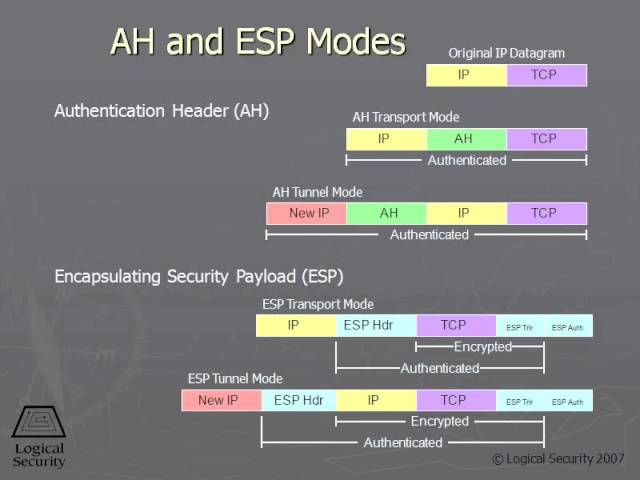
\includegraphics[width=0.86\linewidth]{assets/ipsec_ah_esp_modes.png}

\small\textit{Schéma AH a ESP režimů: AH hlavně autentizuje/integritně chrání, ESP přidává šifrování payloadu; transportní režim chrání původní paket mezi konci, tunelový režim zabalí celý původní IP paket do nového.}
\end{center}

TLS se nachází prakticky mezi transportní a aplikační vrstvou: běží nad TCP a poskytuje bezpečný kanál aplikačním protokolům. Proto vzniká HTTP na HTTPS, FTP na FTPS, případně zabezpečené varianty poštovních protokolů. TLS chrání komunikaci mezi dvěma koncovými body TLS spojení, ověřuje typicky server pomocí certifikátu a po handshake šifruje symetrickým klíčem.

Na aplikační vrstvě existují mechanismy jako PGP nebo S/MIME pro e-mail, aplikační podpisy, tokeny, vlastní autentizační protokoly a aplikační logika. Na linkové vrstvě záleží na technologii: Wi-Fi používá například WPA2/WPA3, podnikové linky mohou mít vlastní linkové zabezpečení, ale není to univerzální ochrana celé internetové cesty.

\itpr{\textbf{Mini box: jak funguje WPA2/WPA3 na Wi-Fi.} WPA chrání bezdrátový úsek mezi klientem a access pointem: nejdřív ověří, že klient zná správné tajemství nebo má správnou identitu, a potom šifruje rámce přenášené vzduchem. U domácího \textbf{WPA2-Personal} mají router i klient stejné heslo/PSK; heslo se neposílá vzduchem, ale použije se při \textbf{4-way handshake}, kde si strany přes nonce odvodí dočasné šifrovací klíče. Data se pak šifrují hlavně pomocí \textbf{AES-CCMP} a kontroluje se integrita, aby útočník nemohl rámce nepozorovaně měnit nebo přehrávat. Slabina WPA2-PSK je, že útočník může zachytit handshake a offline zkoušet hesla ze slovníku. \textbf{WPA3-Personal} nahrazuje PSK handshake metodou \textbf{SAE} (Dragonfly), která je odolnější proti offline hádání hesla a dává každému připojení vlastní klíč s lepší dopřednou bezpečností. Pro firmy je důležitý režim Enterprise, kde se místo sdíleného hesla používá typicky \textbf{802.1X/EAP} a autentizační server.}

VPN znamená virtuální privátní síť. V principu tuneluje provoz přes nedůvěryhodnou síť tak, že mezi klientem a VPN serverem nebo mezi dvěma gatewayemi vznikne chráněný tunel. VPN může chránit důvěrnost a integritu provozu na úseku do VPN brány, umožňuje autentizaci uživatele nebo zařízení a může způsobit, že se klient logicky chová jako součást vzdálené sítě. Neznamená ale automaticky anonymitu ani bezpečnost cílového serveru.

Pokud VPN končí ve firmě, poskytovatel cílové služby stále vidí provoz od VPN brány a aplikace musí být bezpečné samy o sobě.

Firewally filtrují provoz podle pravidel. Paketový filtr pracuje podle IP adres, portů a protokolů na L3/L4. Stateful \textbf{firewall} sleduje stav spojení, takže umí povolit odpovědi k již navázanému spojení. Aplikační firewall nebo NGFW umí kontrolovat obsah aplikačních protokolů, například HTTP, a \textbf{WAF} je specializovaný firewall pro webové aplikace proti útokům jako \textbf{SQL} injection, XSS nebo CSRF.

Proxy funguje jako prostředník: forward \textbf{proxy} řídí odchozí provoz klientů, reverse proxy chrání a zprostředkuje přístup k serverům, často s load balancingem a TLS terminací. \textbf{IDS} útoky detekuje a hlásí, \textbf{IPS} je navíc aktivně blokuje.

Na lokální síti se kromě firewallů uplatňují i ochrany přímo na druhé vrstvě, na switchích. \textbf{DHCP snooping} rozlišuje důvěryhodné a nedůvěryhodné porty a zahazuje DHCP odpovědi z nedůvěryhodných portů, čímž brání podvrženému (rogue) DHCP serveru a omezuje i \textbf{DHCP starvation}, tedy vyčerpání adresního poolu útočníkem. \textbf{Dynamic ARP Inspection} (DAI) kontroluje \textbf{ARP} zprávy proti tabulce z DHCP snoopingu a podvržené zahazuje, čímž brání ARP spoofingu.

Port security omezuje, kolik a jakých \textbf{MAC} adres smí být na portu, a port při porušení zablokuje. Client isolation zabrání tomu, aby spolu klienti na stejné síti, typicky Wi-Fi, navzájem komunikovali. \textbf{VLAN} \textbf{segmentace} odděluje provoz do logických sítí a \textbf{802.1X} vyžaduje autentizaci zařízení nebo uživatele dřív, než se port vůbec zpřístupní.

Dohromady tyto mechanismy řeší útoky, které firewall na hranici sítě nevidí, protože se odehrávají uvnitř jednoho L2 segmentu.

\itbox{\textbf{Vrstvové shrnutí:} Linková vrstva chrání konkrétní linku, IPsec chrání IP komunikaci, TLS chrání kanál pro aplikaci, PGP/S/MIME chrání přímo obsah zprávy. Čím výše zabezpečení leží, tím více rozumí konkrétní aplikaci; čím níže leží, tím transparentnější může být pro aplikace.}

\subsection*{9. Jak bych to celé řekl u státnic}

Síťové aplikace běží na aplikační vrstvě a používají aplikační protokoly, které definují formát, význam a pořadí zpráv. Mezi základní služby patří elektronická pošta, přenos souborů, web a DNS. U pošty se pro odesílání a předávání používá SMTP, zatímco pro vyzvedávání a synchronizaci schránky POP3 nebo IMAP.

U přenosu souborů je klasické FTP nezabezpečené a používá řídicí a datové spojení; FTPS je FTP přes TLS, zatímco SFTP je přenos souborů přes SSH. Web běží nad HTTP, zabezpečená varianta HTTPS používá TLS, které autentizuje server a šifruje komunikaci. DNS je hierarchická distribuovaná služba pro překlad jmen na IP adresy, kde se uplatňuje rekurzivní resolver, root, TLD a autoritativní servery.

Kvalita služby řeší, jaké vlastnosti od přenosu očekáváme: kapacitu, latenci, jitter a ztrátovost. Je důležitá hlavně pro multimédia, VoIP, videokonference a hry, protože ty jsou citlivé na zpoždění a kolísání. Mechanismy QoS zahrnují plánování front, priority, Weighted Fair Queuing, tvarování toků přes Leaky Bucket a Token Bucket a prevenci zahlcení pomocí RED/WRED.

Zabezpečení síťové komunikace řeší důvěrnost, integritu, autentizaci a nepopíratelnost. Symetrická kryptografie je rychlá, ale vyžaduje sdílený klíč; asymetrická kryptografie je pomalejší, ale umožňuje výměnu klíčů a digitální podpisy. V praxi se používá hybridní přístup. Na síťové vrstvě je typický IPsec, mezi transportní a aplikační vrstvou TLS, na aplikační vrstvě například PGP nebo S/MIME.

VPN vytváří chráněný tunel a používá autentizaci a šifrování k ochraně provozu přes nedůvěryhodnou síť.

\subsection*{10. Rychlá kontrola pojmů}

\begin{longtable}{p{0.475\linewidth}p{0.475\linewidth}}
\toprule
\textbf{Oblast} & \textbf{Co říct stručně} \\
\midrule\endhead
SMTP / POP3 / IMAP & SMTP odesílá a předává poštu; POP3 stahuje; IMAP synchronizuje schránku na serveru. \\
\addlinespace
FTP / FTPS / SFTP & FTP je nezabezpečené; FTPS = FTP přes TLS; SFTP = přenos souborů přes SSH; SCP = jednoduché kopírování přes SSH. \\
\addlinespace
DNS & Hierarchie: root, TLD, autoritativní server; rekurzivní resolver dotaz vyřeší a cacheuje. \\
\addlinespace
QoS & Metriky: bandwidth, latence, jitter, ztrátovost; metody: scheduling, token/leaky bucket, RED/WRED. \\
\addlinespace
TLS / IPsec / PGP & TLS chrání kanál aplikace, IPsec IP pakety, PGP/S/MIME obsah e-mailu. \\
\addlinespace
VPN & Tuneluje provoz přes nedůvěryhodnou síť; chrání úsek do VPN brány a autentizuje strany. \\
\addlinespace
\bottomrule
\end{longtable}

\newpage

